%% Preamble
% ---
\documentclass{article}
\usepackage[T1]{fontenc}
\usepackage[utf8]{inputenc}
\usepackage{array}
\usepackage{graphicx}
\usepackage{tikz}
\usetikzlibrary{arrows.meta,positioning,shapes.geometric}
\newcommand{\safeincludegraphics}[2][]{\IfFileExists{#2}{\includegraphics[#1]{#2}}{\fbox{\parbox[c][1.0cm][c]{2.7cm}{\centering\scriptsize College logo file required:\\[2pt]\texttt{#2}}}}}
\newcommand{\missingfigure}[2]{\fbox{\parbox[c][#1][c]{0.88\linewidth}{\centering\textbf{IMAGE REQUIRED}\\[5pt]#2}}}
\tikzset{
  reportbox/.style={draw,rounded corners,align=center,inner sep=6pt,text width=2.6cm,minimum height=0.85cm,font=\small},
  reportsmall/.style={draw,rounded corners,align=center,inner sep=5pt,text width=2.05cm,minimum height=0.75cm,font=\scriptsize},
  reportarrow/.style={-{Latex[length=2mm]},thick},
  reportline/.style={thick}
}
\graphicspath{{./}}
\usepackage{xcolor}
\usepackage[colorlinks]{hyperref}
\usepackage[margin=1in,left=1in,bottom=1in]{geometry}
\usepackage{multicol}
\usepackage{fancyhdr}
\usepackage{setspace}
\usepackage{indentfirst}
\hypersetup{
  colorlinks = true,
  linkcolor  = black
}
\usepackage{tocloft}


\begin{document}

	\begin{center}
		\thispagestyle{empty}
			\safeincludegraphics[width=3cm]{wce_logo.png}
			\\[0.20in]
			\huge \textbf{Walchand College Of Engineering, Sangli.}	\\[0.05in]
\Large  \textbf{(An Autonomous Institute)}
			\\[0.35in]
\textbf{Department Of\\ Computer Science and Engineering}
			%\\[0.30in]\Large \textbf{Year:2026-2027}
			\\[0.30in]{A Project Report \\ On}\\[0.30in]
\LARGE \textbf	{\color{blue}IdleGrid: Distributed Idle/Co-Tenant Compute\\Harvesting Platform for Campus Labs} 
			\\ [0.35in]
			\large	Submitted by\\[0.30in]
\begin{multicols}{2}	
			\textbf{Avadhut Mali\\ (PRN 23510003)}
			\end{multicols}
			\begin{multicols}{2}
		    \textbf{Yash Savalkar\\ (PRN 23510027)}
			\end{multicols} 
			\begin{multicols}{2}
		    \textbf{Krishna Dhumal\\ (PRN 23510057)}
            \end{multicols} 
			\begin{multicols}{2}
		    \textbf{Siddharth Swami\\ (PRN 23510096)}
            
			
			\end{multicols} 
			
			 Under the Guidance \\of \\	
			
			\begin{center}
			\large \textbf{Dr. B.F. Momin\\Department of Computer Science and Engineering\\Walchand College of Engineering, Sangli}
			\\[0.30in]\Large \textbf{Year: 2026 - 2027}
			\end{center}
			%\begin{multicols}
			%\\ \large \textbf{Dr.abc} \\HOD\\Computer Science and Engineering Dept,\\WCE, Sangli.	
			%\end{multicols}
		
			
%\vspace*{\fill}
			% \Large \textbf{May 2017}
	 \end{center}
	\pagebreak
	%\pagestyle{fancy}
	\fancyhf{}
	%\lhead{Time Series Data Analysis for Stock Market Prediction using Data Mining Techniques with R}
	\rfoot{\thepage}
\pagestyle{fancy}
	
	\begin{center}
		\safeincludegraphics[height=4cm]{wce_logo.png}
		\\
		\textbf{\Large Walchand College of Engineering, Sangli}\\
	\Large  (An Autonomous Institute)
\\[0.2in]
\textbf{Department\\ Of\\ Computer Science and Engineering}\\[0.4in]
\LARGE \textbf	{\color{blue}CERTIFICATE } \\[0.4in]
\end{center}


	\par
	\setlength{\parindent}{4em}
	%\doublespacing
	\space
This is to certify that the Project Report entitled, 
\textbf {"IdleGrid: Distributed Idle/Co-Tenant Compute Harvesting Platform for Campus Labs"} submitted by\\
\begin{multicols}{2}
\textbf{Avadhut Mali\\ (PRN 23510003)}
\end{multicols}
\begin{multicols}{2}
\textbf{Yash Savalkar\\ (PRN 23510027)}
\end{multicols}
\begin{multicols}{2}
\textbf{Krishna Dhumal\\ (PRN 23510057)}
\end{multicols}
\begin{multicols}{2}
\textbf{Siddharth Swami\\ (PRN 23510096)}
\end{multicols}
 to Walchand College of Engineering, Sangli, is a record of bona fide Project work carried out by them under my supervision and guidance and is worthy of consideration for the award of the degree of Bachelor of Technology in Computer Science and Engineering of the Institute. 
	

				\vspace{2cm}
\begin{multicols}{2}
	\begin{center}
	\textbf{Dr. B.F. Momin}
	\\ Guide
	\end{center}
	\columnbreak
	\begin{center}
	External Examiner
	\end{center}
\end{multicols}

\vspace{1.5cm}
\begin{center}
	\textbf{Dr. A. R. Surve}
	\\ Head
	\\ Department of Computer Science and Engineering
\end{center}

	\pagebreak
	
	
	\pagebreak
		\pagebreak
	\begin{center}
	\Huge \textbf {\color {blue}Acknowledgement} \\
	\end{center}
	\vspace{1cm}
	{
	\onehalfspacing
	\setlength{\parindent}{2em}
	\setlength{\parskip}{0.8em}

We feel immense pleasure in submitting this project report entitled \textbf{``IdleGrid: Distributed Idle/Co-Tenant Compute Harvesting Platform for Campus Labs''}.

We are thankful to our guide, \textbf{Dr. B.F. Momin}, for the valuable guidance and kind help during the completion of the project.

We are also thankful to the Head of the Department of Computer Science and Engineering, \textbf{Dr. A. R. Surve}, for the valuable guidance during the completion of the project.

We would like to thank all the faculty members and staff of the Department of Computer Science and Engineering for their generous help in various ways in the completion of this project.

We would like to thank all our friends, and especially our classmates, for the thoughtful and mind-stimulating discussions we had, which prompted us to think beyond the obvious. We have enjoyed their companionship so much during our stay at Walchand College of Engineering, Sangli.

	}
	
	\pagebreak
	\begin{center}
		\Huge \textbf{Declaration} \\
	\end{center}
	\vspace{1cm}
	\par 
	\setlength{\parindent}{8em}
	\doublespacing
	\doublespacing
    \noindent
We hereby declare that work presented in this project report titled 
\textbf {"IdleGrid: Distributed Idle/Co-Tenant Compute Harvesting Platform for Campus Labs"}
 submitted by us in the partial fulfillment of the requirement of the award of the degree of \textbf{Bachelor of Technology (B.Tech)} submitted in the \textbf{Department of Computer Science and Engineering, Walchand College of Engineering, Sangli}, is an authentic record of our project work carried out under the guidance of Dr. B.F. Momin, Department of Computer Science and Engineering, Walchand College of Engineering, Sangli.
	

		\begin{multicols}{2}
\textbf{Avadhut Mali\\ (PRN 23510003)}
\end{multicols}
\begin{multicols}{2}
\textbf{Yash Savalkar\\ (PRN 23510027)}
\end{multicols}
\begin{multicols}{2}
\textbf{Krishna Dhumal\\ (PRN 23510057)}
\end{multicols}
\begin{multicols}{2}
\textbf{Siddharth Swami\\ (PRN 23510096)}
\end{multicols}

		\begin{multicols}{2}
		\noindent
		  Date : \\
		  Place : Sangli
		  \flushright{\vspace{1cm}(Signatures)}
		\end{multicols}
	
	\pagebreak
	\begin{center}
	\Large\textbf{ABSTRACT}
	\end{center}
	\noindent
Campus computer laboratories contain PCs whose resources are not always fully used, while students may lack suitable hardware for compute-intensive coursework. IdleGrid is a campus-LAN prototype that coordinates lab PCs through a Spring Boot Master, Windows Agents, Docker Desktop/WSL2, and separate operator and student web interfaces. The Master tracks worker capacity, schedules resource-limited jobs, and stores uploaded files with a primary copy and best-effort worker replicas. Student accounts use file-backed salted password hashes and authenticated sessions; student job, training, and storage history is scoped to the signed-in account. The training area supports two distinct methods: PyTorch DistributedDataParallel (DDP), which requires direct worker connectivity, and coordinator-mediated FedAvg, in which workers upload local model updates to the Master for aggregation. FedAvg supports 2--20 selected workers and includes a 900-image synthetic classification bundle plus a single-PC baseline measurement workflow. The operator dashboard, client application, Master, and Agent are implemented as separate components. Control and session records remain in memory, while uploaded files and metadata are stored on the Master filesystem. This report describes the implemented prototype and its limitations; performance claims are restricted to recorded demonstrations and must be expanded through repeatable lab trials.
	
	\pagebreak
	%\begin{center}
	%	\Huge \textbf{Abstract} \\
	%\end{center}
	%\par
	
	
	%\pagebreak
	\renewcommand{\contentsname}{\textbf{Table Of Contents} }
	\renewcommand{\cfttoctitlefont}{\huge}
	\tableofcontents\thispagestyle{fancy}
	\setlength{\parindent}{4em}
	\setlength{\parskip}{1em}
	\renewcommand{\baselinestretch}{2.0}
	
\listoffigures
\pagebreak
\listoftables
\pagebreak
	\paragraph{Acronyms}
	\begin{itemize}
		\item API \hspace{5em}Application Programming Interface
		\item DDP \hspace{5em}Distributed Data Parallel
		\item FedAvg \hspace{5em}Federated Averaging
		\item Gloo \hspace{5em}Collective communications backend for PyTorch
		\item HTTP \hspace{5em}Hypertext Transfer Protocol
		\item LAN \hspace{5em}Local Area Network
		\item REST \hspace{5em}Representational State Transfer
		\item WSL2 \hspace{5em}Windows Subsystem for Linux 2
		
	\end{itemize}
		
	\pagebreak
	\section{Introduction}
    
Campus laboratories contain computers that are unused at some times or have capacity that is not fully utilized. At the same time, students may have personal devices that are inadequate for compiling large projects, running experiments, processing datasets, or training small machine-learning models. IdleGrid explores whether a campus can make some of its existing computer capacity available through a centrally coordinated, resource-limited service.

The challenge is not simply a shortage of processors. Resources are distributed across multiple PCs, each with a separate operating system, current user, network connection, and local workload. A system that makes the PCs available as one pool must observe the nodes, decide whether a request can fit, tell a worker what to run, bound that work, and present reliable status to the requester. It must also account for the fact that a PC can disappear from the network or become active while a job is running. These characteristics make the project a small distributed-systems problem with both software and operational constraints.

IdleGrid has a Spring Boot Master, Java Agents installed on participating Windows PCs, a React operator dashboard, a separate React student client, and a public Agent download site. Agents report node capacity and pull assigned jobs from the Master. The Master queues ordinary jobs and uses first-fit placement when a node has sufficient reported CPU and memory. Agents run assigned workloads in Docker containers with CPU and memory limits. The operator dashboard provides management views for nodes, jobs, bookings, shared storage, DDP, and FedAvg. The student client provides basic account login and user-scoped jobs, storage, and training history.

The Master is a control plane rather than a worker. It receives browser requests, records node and job state, schedules eligible ordinary jobs, and makes assignments available to Agents. The Agent reports capacity, polls for work, launches and watches containers, captures output, and informs the Master about completion. Student requests pass through authenticated client APIs that enforce ownership of jobs and uploaded files. Agents initiate assignment requests using a request/poll pattern.

The implementation also includes a shared-file workflow and two CPU-based distributed-training workflows. The DDP mode reserves two or three workers and runs one rank per worker; user code handles data partitioning and gradient synchronization. The separate FedAvg mode supports 2--20 selected workers and transfers local model updates through the Master. The built-in demo bundle contains 900 synthetic images and, when run, measures a single-PC full-data baseline after aggregation. These features depend on Windows/WSL2/Docker configuration and campus network behavior; only DDP requires direct worker-to-worker training connections.

This project should be understood as a prototype rather than a production cloud. Node, job, booking, session, and training-run control records are held in memory and are lost when the Master restarts. Student account hashes and account records are file-backed; student sessions, job ownership, and per-user training history are in memory. File content and its index are stored on the Master filesystem. Production identity integration, durable job records, checkpointing, replica repair, and a fairness-aware scheduler remain future work.

This report describes implemented behavior and distinguishes it from future work. It includes one recorded FedAvg demonstration result, but does not infer general performance from that single run. The following chapters review related work, identify the gap, specify stakeholders and objectives, describe the system design and algorithms, and present a reproducible evaluation plan. The remaining screenshots, hardware details, repeat measurements, and signatures are identified for the project team to provide.

	\subsection{Problem Statement}

Campus computer laboratories are shared environments rather than dedicated datacenters. Their machines have finite CPU, memory, and disk resources, fluctuate in availability, and must remain usable by their owners. A compute-pooling system must therefore discover participating PCs, keep their status current, match requests to capacity, limit the impact of running workloads, and handle node or network failure. These requirements make resource aggregation more than simply launching a command on a remote computer.

In the current prototype, a central Master maintains node and job records in memory. Agents send heartbeats, and a scheduler assigns a queued job to the first online node whose reported free CPU and memory meet the request. An Agent pulls the assignment and starts a resource-capped container. This centralized first-fit method is intentionally simpler than fairness-aware or datacenter-scale schedulers; it is appropriate for demonstrating a small trusted lab prototype but does not guarantee fairness or globally optimal placement. Figure~\ref{fig:problem-context} illustrates the resource mismatch addressed by the project.

The system has to make decisions from periodically reported data. A heartbeat gives the Master a snapshot, not a guarantee that reported free resources will remain available until a container starts. Users may submit requests that exceed capacity; these should remain queued or be rejected according to the workflow. A worker can lose its Master connection, a container can exit unsuccessfully, or a DDP peer can be unreachable even when an Agent can contact the Master. FedAvg avoids peer networking, but still depends on each worker maintaining HTTP access to the Master.

There is also a machine-ownership constraint. A lab PC may be used for teaching or administrative work while a background computation is running. Container CPU and memory caps limit the resources allocated to an individual container, but do not prove that the owner will experience no slowdown. The Agent can detect a return to activity and stop an active workload; this is a coarse protection mechanism because it ends the container and does not preserve progress. The report therefore treats foreground responsiveness as something to measure rather than a guaranteed outcome.

\begin{figure}[htbp]
\centering
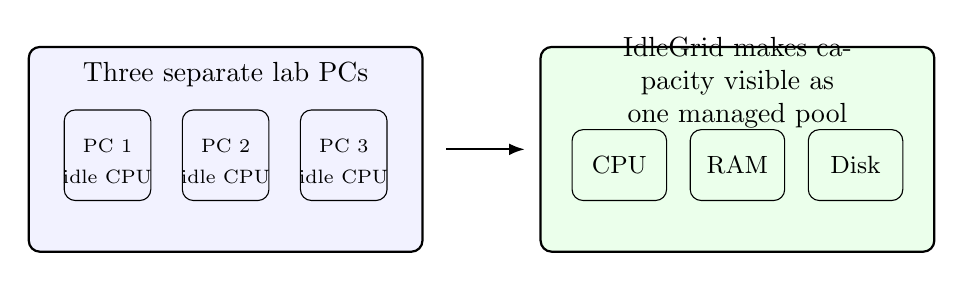
\begin{tikzpicture}[x=1cm,y=1cm]
  \draw[thick,rounded corners,fill=blue!5] (0,0) rectangle (5.0,2.6);
  \node[align=center,text width=4.3cm] at (2.5,2.25) {Three separate lab PCs};
  \foreach \x/\lab/\cpu in {0.45/PC 1/idle CPU,1.95/PC 2/idle CPU,3.45/PC 3/idle CPU}{
    \draw[rounded corners] (\x,0.65) rectangle +(1.1,1.15);
    \node[align=center,font=\scriptsize] at (\x+0.55,1.35) {\lab};
    \node[align=center,font=\scriptsize] at (\x+0.55,0.95) {\cpu};
  }
  \draw[reportarrow] (5.3,1.3) -- (6.3,1.3);
  \draw[thick,rounded corners,fill=green!8] (6.5,0) rectangle (11.5,2.6);
  \node[align=center,text width=4.3cm] at (9,2.15) {IdleGrid makes capacity visible as one managed pool};
  \foreach \x/\lab in {6.9/CPU,8.4/RAM,9.9/Disk}{
    \draw[rounded corners] (\x,0.65) rectangle +(1.2,0.9);
    \node[align=center,font=\small] at (\x+0.6,1.1) {\lab};
  }
\end{tikzpicture}
\caption{Conceptual resource mismatch motivating IdleGrid.}
\label{fig:problem-context}
\end{figure}

\textbf{Problem statement:} Design and prototype a campus-LAN platform that discovers participating Windows PCs, monitors their available resources, assigns user-submitted compute jobs to eligible nodes, and executes those jobs within per-container CPU and memory limits, while supporting shared files and a small multi-node training workflow. The system must expose its operation through a web dashboard and accurately report failure and scope limitations. The principal challenges are dynamic node availability, imperfect capacity estimates, non-interference with PC owners, network reachability, and limited persistence and fault recovery.

	
	\subsection{Motivation}

Students who do not own high-performance computers can face barriers when completing compute-intensive coursework. A campus lab already contains machines with useful CPU and memory capacity, but that capacity is not necessarily accessible outside scheduled lab use. A controlled pool could make those resources easier to discover and use without purchasing a separate compute cluster for every student. The potential benefit is reuse of existing equipment, not a claim that the lab has unlimited or cost-free capacity: electricity, administration, maintenance, bandwidth, and staff time remain real costs.

The project is relevant to students, teaching staff, and lab administrators. Students need a simple way to view availability and submit jobs without learning a separate remote-execution interface for every PC. Teaching staff may benefit from a repeatable environment for demonstrations and small experiments, particularly where a lab exercise involves distributed execution. Administrators need visibility into participating nodes, bounded workloads, and clear operational requirements before approving any installation. The public Agent download page can simplify distribution, but it does not replace installation review, endpoint policy, or administrator approval.

IdleGrid is also a practical learning exercise in distributed systems: it combines heartbeats, scheduling, container execution, file replication, web APIs, failure detection, student account boundaries, DDP, and FedAvg. Heartbeats make liveness observable; polling limits the need for the Master to initiate worker connections; first-fit gives a simple placement baseline; containers apply per-workload limits; DDP demonstrates direct communication requirements; and FedAvg demonstrates coordinator-mediated model aggregation.

The student client provides basic account login and restricts client job, training-history, and uploaded-file views to the signed-in account. This is a prototype identity boundary, not a production identity service. The operator dashboard and most Master APIs remain suitable only for a trusted, controlled network; storage access keys also grant access to their corresponding files. These constraints should be considered before any campus deployment beyond an approved demonstration.

    \subsection{Significance of the problem}
	
IdleGrid uses a centralized control plane and lightweight worker Agents. The Master is the single point through which the dashboard and Agents coordinate. This design provides a clear source of node and job status and simplifies a small prototype compared with a decentralized membership and scheduling protocol. Its first-fit scheduler is easy to inspect and demonstrate, although it is not intended to provide fairness, optimal packing, or production-scale throughput.

The implementation combines ordinary batch jobs with shared-file handling and two distinct training workflows. DDP synchronizes gradients directly among workers and requires peer connectivity. FedAvg lets workers train locally and exchange model updates through the Master, so workers do not need direct connections to each other. Docker CPU and memory limits bound each ordinary container, while Agent activity detection and job eviction provide a basic response when a user returns after an idle period. Eviction is a failure rather than a checkpoint-and-resume operation. The project is a resource-capped lab-compute prototype, not a fully elastic co-tenant scheduler.

The significance of the work is the integration of these capabilities into a single campus-oriented prototype and the opportunity to measure them on real lab equipment. The design combines separate operator and student interfaces, a central coordination service, worker-side Agents, and a container runtime. It includes complete request paths from authenticated student submission to worker execution and returned status, file storage, DDP, and coordinator-mediated FedAvg.

The principal engineering contribution is integration for a constrained environment: Windows PCs using Docker Desktop and WSL2, a campus LAN, a small node count, and a single central Master. The use of a simple first-fit scheduler keeps placement behavior understandable and supports a baseline implementation against which a future fairness-aware strategy could be evaluated. The use of Docker resource limits gives a concrete mechanism for restricting per-job CPU and memory, while the Agent's activity detector supplies a separate return-to-use response. These mechanisms address different aspects of resource management and should not be conflated: one limits container allocation, while the other can terminate a job after renewed user activity.

The project should be evaluated by measuring rather than assuming its benefits. Evaluation should vary worker count, job CPU and memory requests, workload duration, and worker availability. Metrics include queue-to-assignment delay, job makespan, completion ratio, throughput, utilization, replica completion, DDP artifact success, and FedAvg comparison against a single-PC baseline. Owner impact should be measured using a controlled foreground task. Repeated trials are required because startup, image availability, transfer, background load, and thermal conditions affect measurements.

No numerical results are included here because the project documentation does not provide recorded measurements. Accordingly, the report does not claim an improvement over cloud services, existing schedulers, idle-only systems, or a baseline implementation. The Results and Analysis section contains a test matrix and data-collection structure that must be completed from actual runs. Once measurements are collected, they can establish whether the prototype meets its local functional goals and under which test conditions its resource-pooling approach is useful.

	\pagebreak
    
	\section{Literature Review and Research Gap}
The relevant background includes idle-workstation harvesting, volunteer computing, cluster scheduling, container orchestration, and multi-node machine learning. These areas offer useful design patterns, but their assumptions differ from a small Windows-based campus lab.

Condor established the idea of matching computation to idle workstations and is a foundational example of cycle harvesting \cite{condor}. BOINC extended volunteer computing to large pools of independently operated computers, emphasizing client-side participation and fault tolerance \cite{boinc}. These systems demonstrate that distributed spare capacity can be useful, but a campus deployment also needs straightforward local administration, current resource visibility, and a clear way to run containerized coursework workloads.

Cluster schedulers address placement and resource allocation at a larger scale. Dominant Resource Fairness provides a principled way to allocate multiple resource types fairly \cite{drf}, while the Borg experience describes production scheduling and container management at datacenter scale \cite{borg}. IdleGrid currently uses a simpler first-fit policy rather than these more advanced strategies. This keeps placement behavior understandable for a small prototype, but makes fairness and allocation efficiency important future evaluation and development topics.

Container-based co-location work, including Bubble-Up and Heracles, studies the interference that occurs when workloads share hardware and the mechanisms used to control it \cite{bubbleup,heracles}. IdleGrid applies per-container CPU and memory limits and records Windows idle/active transitions, but its implementation does not include feedback-driven interference control. An Agent may evict a running job after a return-to-active transition, and the job is reported as failed rather than resumed. Thus the current design is a practical baseline for experimentation, not a demonstration that user experience is unaffected.

PyTorch DDP supplies a data-parallel training model in which separate processes synchronize gradients; a distributed sampler can assign different training examples to each rank \cite{pytorchddp}. IdleGrid includes this DDP orchestration path and a separate coordinator-mediated FedAvg path. In the FedAvg demo, each worker selects its own deterministic shard from a common 900-image synthetic dataset, performs local training, and uploads a model update to the Master. FedAvg avoids direct worker-to-worker networking but is a single-round prototype, not a general-purpose distributed training framework.

The systems and concepts reviewed above differ in target scale and assumptions. Condor and BOINC demonstrate resource harvesting and volunteer participation, but their history and operating models do not directly prescribe how a department should deploy a Windows Agent, configure Docker Desktop, and expose a browser dashboard on a private campus LAN. Borg and DRF address larger shared clusters and multi-resource allocation; they provide useful comparison points but would add complexity beyond the current project's first-fit scope. Co-location studies focus on measuring and controlling interference, which makes owner responsiveness an important experiment rather than something that can be inferred from resource caps alone.

\begin{table}[h!]
\centering
\caption{Comparison of related approaches with the IdleGrid prototype.}
\label{tab:related-work}
\begin{tabular}{|p{0.16\linewidth}|p{0.26\linewidth}|p{0.24\linewidth}|p{0.24\linewidth}|}
\hline
Approach & Main focus & Relevance to this project & Difference from current IdleGrid \\
\hline
Condor \cite{condor} & Harvesting cycles from idle workstations & Establishes workstation resource harvesting as a systems problem & IdleGrid is a small campus-LAN prototype with dashboard-based submission and Docker jobs \\
\hline
BOINC \cite{boinc} & Public-resource and volunteer computing & Demonstrates large-scale participation and distributed task execution & IdleGrid assumes a managed lab environment and central Master; it is not a public volunteer network \\
\hline
DRF \cite{drf} & Fair allocation of multiple resource types & Provides a candidate future scheduler and evaluation baseline & Current ordinary placement uses first-fit and does not provide DRF fairness guarantees \\
\hline
Borg \cite{borg} & Large-scale cluster orchestration & Provides context for resource reservation and container management & IdleGrid targets a handful of Windows PCs, not datacenter-scale workloads \\
\hline
Bubble-Up / Heracles \cite{bubbleup,heracles} & Co-location interference and resource efficiency & Motivates controlled measurement of worker-owner impact & IdleGrid has limits and activity-based eviction, but no feedback controller or proven zero-impact guarantee \\
\hline
PyTorch DDP \cite{pytorchddp} & Synchronous data-parallel model training & Supplies the training primitive used by the multi-worker demonstration & IdleGrid coordinates workers; the user script implements model, sampler, and synchronization logic \\
\hline
\end{tabular}
\end{table}

\textbf{Identified gap:} the referenced systems provide important foundations, but do not by themselves document an integrated, small-scale campus prototype combining separate operator and student interfaces, Windows Agents, Docker/WSL2 execution, first-fit placement, shared file replicas, DDP, and coordinator-mediated FedAvg. IdleGrid's contribution is this integration and its concrete evaluation opportunity. It is not claimed to outperform Condor, BOINC, or datacenter schedulers.

\textbf{Positioning and research questions.} The project can be evaluated through questions that match the implementation: (1) Can a node heartbeat and job request pass through the Master--Agent--container lifecycle? (2) How do queue delay and makespan change with worker count and resource request? (3) Under what conditions do worker file replicas complete? (4) Can DDP complete when peer traffic is permitted? (5) How does coordinator-mediated FedAvg compare with the same single-PC workload as worker count changes? (6) What observable change in foreground responsiveness occurs under a capped workload? These questions avoid claiming novelty in first-fit scheduling itself.
    \pagebreak
    \section{Customer Details and Use Cases}
The primary customers are students who need temporary compute resources for coursework and small experiments but do not have suitable local hardware. Secondary stakeholders are instructors who demonstrate distributed or containerized workloads and laboratory administrators responsible for approving software and network access. The current prototype assumes a trusted campus LAN and administrator approval for installing Java, Docker Desktop, WSL2, and the Agent.

The stakeholder roles have different requirements. A student needs understandable resource choices, clear job status, and access to output without knowledge of the worker's local configuration. The separate client includes basic login and user-scoped job, training, and storage history. An instructor needs a reproducible demonstration and a way to determine whether a job actually completed. A laboratory administrator needs to understand installation privileges, ports, Docker/WSL2 configuration, resource ceilings, and the effect of worker shutdown. The prototype has no production-grade administrator policy console or identity provider.

\textbf{Use case 1 -- Submit a batch job:} A student opens the dashboard, selects a command and CPU/RAM request, and submits it. The Master queues and attempts to place the job. The selected Agent polls for an assignment, starts a Docker container, captures its output, and reports completion. The dashboard displays job status and final output; it is not a live interactive terminal.

\textbf{Use case 2 -- Store and retrieve a file:} A signed-in student uploads a file in the client Storage page. The Master stores the primary copy, associates the record with the student account, and returns a file access key. Eligible online Agents may store up to two replicas. The client lists and downloads only files owned by the signed-in student.

\textbf{Use case 3 -- Run distributed training:} An operator can choose either DDP or coordinator-mediated FedAvg. DDP launches ranks on two or three workers and needs direct worker connectivity. FedAvg distributes data slices to 2--20 workers, receives local checkpoints through the Master, and combines them with sample-weighted averaging. The FedAvg demo also runs a full-data single-PC baseline on rank zero and records both timing and model metrics.

\textbf{Use case 4 -- Monitor lab capacity:} A lab administrator or instructor views node status and reported CPU, memory, and disk capacity in the dashboard and checks whether Agents are reaching the Master.

\textbf{Use case 5 -- Request a targeted session:} A user selects an online node and requests a time-limited SSH-enabled container session through the Book Resources workflow. The backend creates a target-node job and constructs the session command; the requested duration is capped at 24 hours. This is a containerized workload path, not SSH access to the Windows host. The booking records exposed through the booking API are in-memory records and do not implement a durable calendar or reservation guarantee.

\textbf{Use case 6 -- Recover from unavailable capacity:} If no online worker meets the CPU/RAM request, an ordinary job remains queued. The user can inspect its status while the scheduler retries on later passes. The prototype does not guarantee a wait time or fairness among users. If a node becomes stale, the Master marks it offline after the heartbeat timeout and applies the implemented requeue behavior for affected ordinary jobs; DDP worker loss fails the coordinated run.

\textbf{Use-case boundary:} This report describes authorized prototype use on a trusted campus network. Student accounts provide basic per-user separation for client jobs, training history, and uploaded files; this is not a production identity, billing, quota, or enterprise authorization system. Public API exposure and guaranteed long-running services are outside scope.
	\pagebreak
	\section{Project Objectives}
    \begin{enumerate}
      \item To design and implement a centralized platform for monitoring compute resources on campus laboratory PCs.
      \item To enable submission, first-fit scheduling, and Docker-based execution of CPU- and memory-constrained jobs.
      \item To provide a shared-file workflow with a Master-stored primary copy and best-effort worker replicas.
  \item To provide a separate authenticated student client with user-scoped jobs, storage, and training history.
  \item To implement CPU-based DDP and coordinator-mediated FedAvg training workflows, including a single-PC comparison report for FedAvg.
      \item To define and conduct controlled measurements of job execution, resource use, storage replication, and worker availability.
    \end{enumerate}
	\pagebreak	
	\section{Proposed Method and Algorithm}
The problem is to accept a compute request and place it on an eligible campus PC while keeping the worker, job, and user-visible status coordinated. A solution must account for delayed or missing heartbeats, resource requests that exceed all reported capacity, Agent polling intervals, and the difference between ordinary batch work and coordinated multi-node training. IdleGrid addresses these constraints with a central Master, periodic heartbeats, a first-fit scheduler for ordinary jobs, pull-based Agent assignments, and separate gang placement for DDP runs. The current solution favors simplicity and traceability over fairness, durability, and optimal placement.

	\subsection{Problem Definition}

Given a set of worker nodes \(N\), each with a reported online state and free CPU and memory, and a user job request \(J=(c_j,m_j,\mathrm{command},\mathrm{image})\), the Master selects an eligible node whose reported capacity satisfies the request, or leaves the job queued. For DDP, the inputs include a validated training bundle, worker count, resource requests, image, and output filename; success requires the program to synchronize ranks over direct worker connections and upload the rank-zero artifact. For FedAvg, workers train local data shards and upload model updates to the Master; rank zero computes a sample-weighted aggregate, then measures a single-PC run on the full dataset for comparison.

The ordinary-workload input can include an optional target node and an optional duration for a time-limited SSH-style container session. A request also depends on the worker having access to the selected container image and a usable workspace. The platform does not accept a generic high-level program and infer its parallelism: for distributed training, the uploaded ZIP must contain a compatible Python entry point and the command supplied by the user must be valid in the training container. The run request specifies a worker count of two or three and a requested amount of CPU and memory for each selected worker.

The output is not limited to whether the command started. The Master exposes job and training states; the Agent returns the container result and captured output when ordinary execution completes; training reports include per-worker state, metrics, and timing. DDP produces its rank-zero model artifact; FedAvg provides an aggregated model and a structured one-PC comparison. Student client storage lists only the signed-in student's uploads, while operator shared storage uses the operator API. Replica acknowledgements remain distinct from the Master primary copy.

The objective is to demonstrate end-to-end resource monitoring, placement, execution, and status reporting on a campus LAN. Constraints include Windows worker PCs, Java 17+, Docker Desktop with WSL2, and network access to the Master. Direct worker-to-worker TCP connectivity is required for DDP but not for FedAvg. Node, job, booking, session, and training-run state is in memory; student account hashes are file-backed; student file bytes and metadata are stored on the Master filesystem. Capacity reports may become stale, first-fit is not a fairness policy, and ordinary job output is available after completion rather than as a live terminal. The prototype should remain on an approved trusted network.

	\subsection{Proposed Idea/System}
The core idea is to turn existing lab PCs into visible worker nodes without making the browser communicate directly with each PC. The operator dashboard and student client submit requests to the Master, the Master tracks worker heartbeats and job state, and each Agent pulls its own assignment. Docker enforces per-job CPU and memory limits at container launch. Student records are scoped to authenticated accounts in the client workflow.

The first-fit scheduler walks online nodes and assigns a queued job to the first node with sufficient reported CPU and memory after accounting for active reservations. Heartbeats older than the configured timeout cause a node to be marked offline. Jobs affected by node loss may be requeued according to the Master workflow; no checkpoint is created. For shared files, the Master stores the authoritative file and metadata and queues replica tasks for eligible workers. DDP placement reserves a complete two- or three-worker group and launches synchronized ranks. FedAvg selects 2--20 eligible workers, trains local data partitions, and has rank zero average worker checkpoints after retrieving them through HTTP. The novelty claimed here is the integrated, lab-focused prototype and its workflow, not a new scheduling algorithm.
    
	\subsection{System Architecture}
IdleGrid uses a centralized architecture. The operator dashboard and authenticated student client call the Spring Boot Master over HTTP. The Master maintains in-memory node and job control state, account sessions, and run histories; it stores primary files and a JSON metadata index on its filesystem. Java Agents on Windows PCs report heartbeats and pull jobs or storage tasks. Assigned jobs run in Docker Desktop containers through WSL2. DDP workers require direct peer-to-peer connectivity, while FedAvg workers communicate with the Master to upload and download checkpoints. Figure~\ref{fig:architecture} shows these paths; the implementation description follows the project technical guide \cite{idlegridguide}.

\textbf{Web applications.} IdleGrid has an operator dashboard and a separate React student client. The operator interface includes node monitoring, job management, storage, bookings, DDP, and coordinator-mediated FedAvg. The student client has basic login and student-facing capacity, job submission, training history, and storage views; the backend filters the student's jobs and uploaded files by the authenticated account. The public download site is a third, separate application that serves the portable Agent ZIP. Browser applications call the Master API and do not run Docker directly on workers.

\textbf{Master service.} The Master is implemented in Java with Spring Boot. Controllers expose node, job, booking, storage, client-authentication, DDP, and FedAvg endpoints. The scheduler evaluates ordinary queued jobs and reserves worker groups for training. Student account password hashes are held in a local account file; session, job-ownership, and training-history state is in memory. File bytes and a JSON index are stored under the configured filesystem directory, while training bundles and artifacts are stored under the configured training directory. The Master advertises its LAN endpoint through rendezvous and local discovery mechanisms. It remains a single coordination point, and in-memory state is not recovered after restart.

\textbf{Worker Agent.} A Java background process runs on each participating Windows PC. Scheduled tasks send heartbeats, check Windows input inactivity, poll for job assignments, monitor running containers, and request storage replication tasks. The Agent keeps a stable node identifier in a local file unless explicitly configured otherwise. It launches jobs using Docker CLI commands, captures session output in local logs, and reports running/completed status to the Master. The Agent is packaged as a portable ZIP with a launcher, configuration, and setup helper; Java 17+ and Docker Desktop/WSL2 are runtime requirements.

\textbf{Container runtime and data paths.} Ordinary jobs run in Docker containers with CPU and memory limits and a per-job workspace mounted at \texttt{/workspace}. Ordinary and FedAvg containers use Docker bridge networking; FedAvg workers communicate only with the Master. DDP containers use the configured host networking because rank processes must communicate directly. Docker Desktop uses WSL2 on the Windows worker. This deployment depends on installed versions, Docker configuration, firewall policy, and campus network topology.

\textbf{Storage component.} The Master maintains a canonical file copy and JSON metadata index. After an upload, it may queue up to two replica tasks on online Agents with available disk. Agents poll, download the source bytes from the Master, write local copies, and acknowledge completion. This is not a distributed object store: the repository does not implement MinIO, S3, erasure coding, user buckets, or a repair/rebalance service. DDP bundles and output artifacts follow their own training-run paths and have separate validation and size constraints.

\textbf{External communication and ports.} The HTTP Master API uses TCP port 9090 by default. Local Agent discovery uses UDP port 9091. DDP uses its configured rendezvous port (29500 by default) and additional peer connections. Agents and FedAvg workers must reach the Master; DDP additionally requires direct worker-to-worker connectivity. A successful heartbeat therefore does not prove that DDP peer traffic is available.

\begin{figure}[htbp]
\centering
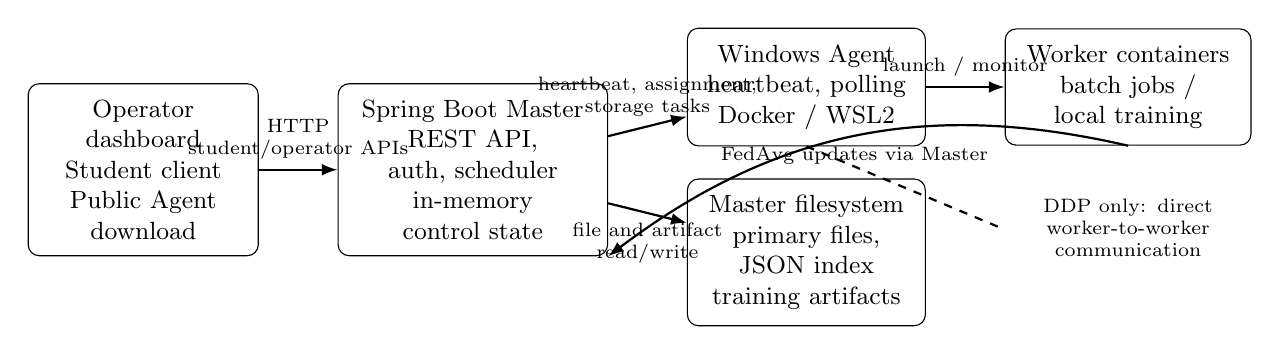
\begin{tikzpicture}[node distance=1.25cm and 1.0cm]
  \node[reportbox,text width=2.5cm] (web) {Operator dashboard\\Student client\\Public Agent download};
  \node[reportbox,text width=3.0cm,right=of web] (master) {Spring Boot Master\\REST API, auth, scheduler\\in-memory control state};
  \node[reportbox,text width=2.6cm,right=of master,yshift=1.05cm] (agent) {Windows Agent\\heartbeat, polling\\Docker / WSL2};
  \node[reportbox,text width=2.6cm,right=of master,yshift=-1.05cm] (files) {Master filesystem\\primary files, JSON index\\training artifacts};
  \node[reportbox,text width=2.7cm,right=of agent] (container) {Worker containers\\batch jobs / local training};
  \draw[reportarrow] (web) -- node[above,font=\scriptsize,align=center]{HTTP\\student/operator APIs} (master);
  \draw[reportarrow] (master) -- node[above,font=\scriptsize,align=center]{heartbeat, assignment,\\storage tasks} (agent);
  \draw[reportarrow] (agent) -- node[above,font=\scriptsize,align=center]{launch / monitor} (container);
  \draw[reportarrow] (master) -- node[below,font=\scriptsize,align=center]{file and artifact\\read/write} (files);
  \draw[reportarrow] (container.south) to[bend right=25] node[below,font=\scriptsize]{FedAvg updates via Master} (master.south east);
  \node[below=0.55cm of container,align=center,font=\scriptsize,text width=3cm] (peer) {DDP only: direct worker-to-worker communication};
  \draw[reportline,dashed] (agent.south) -- (peer.west);
\end{tikzpicture}
\caption{High-level architecture of the IdleGrid prototype.}
\label{fig:architecture}
\end{figure}

	\subsection{System Analysis and Design}
The design follows the repository's implemented API boundaries and operating assumptions. The subsections below list functional and non-functional requirements, explain the main workflow, define test cases for execution, and summarize the placement algorithm. Tests are described as planned/expected checks; their results must be recorded during actual runs.
	%\pagebreak
	\subsubsection{Requirement Specification}
\textbf{Functional requirements:}
\begin{enumerate}
  \item The Master shall accept Agent heartbeats and expose node status and reported capacity to the dashboard.
  \item A user shall be able to submit a job with a command and CPU/memory request and inspect its state and completion output.
  \item An Agent shall pull an assignment, start a resource-limited Docker container, and report job completion or failure.
  \item A user shall be able to upload and download shared files using a generated access key; eligible worker nodes may store replicas.
  \item A student shall authenticate through the client and see only that account's jobs, training history, and uploaded files.
  \item An operator shall be able to submit and inspect a DDP run on two or three workers and retrieve its artifact when produced.
  \item An operator shall be able to submit coordinator-mediated FedAvg on 2--20 eligible workers, compare it with a single-PC baseline, and download the run report and aggregate model.
\end{enumerate}
\textbf{Non-functional requirements and constraints:} Java 17 or later is required for the backend and Agent; worker PCs require Windows, Docker Desktop, and WSL2. The applications are browser-based. Agents and FedAvg containers must reach the Master; DDP additionally requires worker-to-worker TCP connectivity and compatible networking. Capacity values are periodic estimates. Client sessions and job/run ownership are in memory and there is no checkpoint-based restart; the system should be restricted to an approved trusted network.

Table~\ref{tab:requirements} makes the requirements traceable to observable behavior. Priorities describe the prototype's intended functional importance, not a contractual production service level.
\begin{table}[h!]
\centering
\caption{Functional and operational requirement traceability.}
\label{tab:requirements}
\begin{tabular}{|p{0.1\linewidth}|p{0.43\linewidth}|p{0.24\linewidth}|p{0.12\linewidth}|}
\hline
ID & Requirement & Verification evidence & Priority \\
\hline
FR1 & Register/update nodes from Agent heartbeats and expire stale presence & Node summary and heartbeat test & High \\
\hline
FR2 & Accept a job with CPU, memory, command, optional image and target & Job API response and dashboard & High \\
\hline
FR3 & Place a job only when an online node meets reported CPU/RAM & Assignment status and scheduler logs & High \\
\hline
FR4 & Execute an assignment in a bounded Docker container & Agent log and container inspection & High \\
\hline
FR5 & Return status and completion output to the Master & Job status endpoint and dashboard & High \\
\hline
FR6 & Store file content on Master and expose key-based retrieval & Upload/download checksum comparison & Medium \\
\hline
FR7 & Schedule eligible worker replicas and track acknowledgements & Storage page and Agent logs & Medium \\
\hline
FR8 & Reserve 2--3 workers for DDP and expose rank status/artifact & Run status and rank-zero artifact & Medium \\
\hline
FR9 & Authenticate students and scope client jobs, files, and training history to each account & Two-account access-control check & High \\
\hline
FR10 & Run FedAvg on 2--20 workers and record a single-PC baseline comparison & Run report and model artifact & High \\
\hline
NFR1 & Operate within approved Windows/WSL2/Docker campus environment & Deployment record & High \\
\hline
NFR2 & Keep user-facing pages separate from per-node execution & Architecture and API trace & High \\
\hline
NFR3 & Make failure and prototype limitations explicit to operators & Logs, status and report caveats & High \\
\hline
NFR4 & Keep operator APIs on an approved trusted network and protect client account data & Deployment review & Critical \\
\hline
\end{tabular}
\end{table}

	\subsubsection{Flowcharts, Data Flow, and Functional Design}
The ordinary job data flow is: user submits a request to the dashboard; the dashboard sends it to the Master; the Master queues and attempts first-fit placement; the selected Agent polls and receives the assignment; Docker runs the container; and the Agent sends completion status and output to the Master for dashboard display. If no node meets the request, the job remains queued. Figure~\ref{fig:job-flow} depicts this lifecycle.

The heartbeat path runs independently of job submission. At its configured interval, each Agent samples local information and sends a heartbeat containing its node identity, IP address, CPU and memory totals/free values, disk information, and status. The Master updates the node record and last-seen time. A stale heartbeat eventually causes the node to be considered offline. This mechanism provides liveness information but is not a continuous resource reservation: the host may change resource use between measurements.

The storage path begins when the browser uploads a multipart file to the Master. The Master stores the file and associates it with a randomly generated key in the JSON index. Where disk capacity permits, the storage service queues replica work. An Agent pulls a replica task, fetches the primary content, writes it to its configured storage directory, and sends a completion acknowledgement. The primary Master copy remains the authoritative source. If an Agent is offline or does not have enough disk, a worker replica may not be created.

The DDP path differs from an ordinary job because a run requires a group of workers to start coordinated ranks. The Master validates the archive and request, reserves eligible PCs, and creates a rank assignment for each. The user's script initializes Gloo, partitions examples, and wraps the model using DDP. Rank zero uploads the final artifact. A rank or peer-network failure can fail the group; there is no checkpoint-based recovery.

The FedAvg path is coordinator-mediated. The Master reserves 2--20 eligible PCs and starts one local training task per worker. Every worker downloads the same bundle, uses its rank and the requested world size to select a non-overlapping shard, trains locally, and posts its checkpoint to the Master. Rank zero waits for all updates, downloads them, performs sample-weighted averaging, and uploads the aggregate artifact. The same rank-zero machine then trains on the complete dataset as a single-PC baseline. Thus its comparison report distinguishes the baseline training duration, distributed phase duration, and overall elapsed run duration. A single successful run demonstrates this workflow, but does not by itself establish a general speedup.

\textbf{Logical data-flow boundary.} The browser exchanges HTTP requests and responses with the Master. Agents exchange heartbeats, assignment polls, job state updates, and storage replica messages with the Master. FedAvg containers also use the Master for bundle and checkpoint transfers; DDP containers exchange training traffic directly with peer workers. A successful heartbeat validates only Agent-to-Master reachability, not DDP peer connectivity. The user's browser never opens an execution channel to a worker.

\begin{figure}[htbp]
\centering
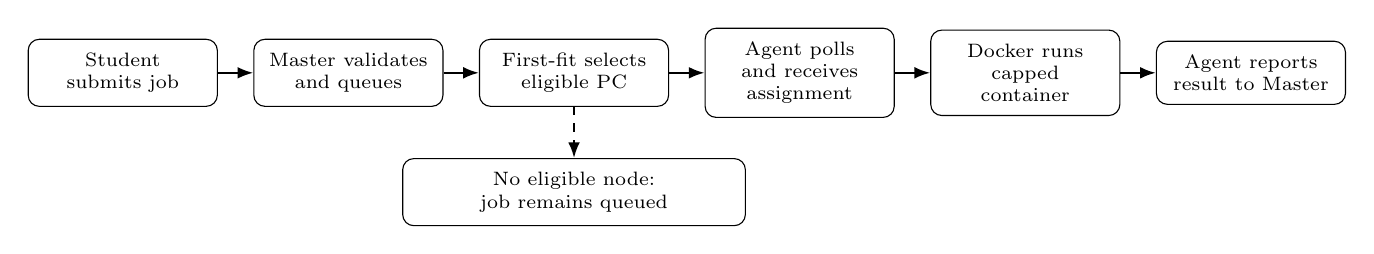
\begin{tikzpicture}[node distance=0.55cm and 0.45cm]
  \node[reportsmall] (submit) {Student submits job};
  \node[reportsmall,right=of submit] (api) {Master validates and queues};
  \node[reportsmall,right=of api] (schedule) {First-fit selects eligible PC};
  \node[reportsmall,right=of schedule] (agent) {Agent polls and receives assignment};
  \node[reportsmall,right=of agent] (docker) {Docker runs capped container};
  \node[reportsmall,right=of docker] (result) {Agent reports result to Master};
  \draw[reportarrow] (submit) -- (api);
  \draw[reportarrow] (api) -- (schedule);
  \draw[reportarrow] (schedule) -- (agent);
  \draw[reportarrow] (agent) -- (docker);
  \draw[reportarrow] (docker) -- (result);
  \node[below=0.65cm of schedule,reportsmall,text width=4cm] (queued) {No eligible node: job remains queued};
  \draw[reportarrow,dashed] (schedule) -- (queued);
\end{tikzpicture}
\caption{Ordinary job submission, placement, and execution workflow.}
\label{fig:job-flow}
\end{figure}

	\subsubsection{Design and Test Cases}
Table~\ref{tab:testcases} lists functional checks that should be executed in a controlled environment. The expected behavior is derived from the documented API and workflows; the observation column must be completed from actual tests. Before each test, record the software versions, node identifiers, network configuration, and whether images are already cached. This avoids mistaking an image-pull delay or a network policy issue for scheduler performance.
\begin{table}[h!]
\centering
\caption{Functional test cases and observations to be recorded.}
\label{tab:testcases}
\begin{tabular}{|p{0.08\linewidth}|p{0.25\linewidth}|p{0.35\linewidth}|p{0.2\linewidth}|}
\hline
ID & Scenario & Expected result & Observation \\
\hline
TC1 & Agent heartbeat & Node appears online with reported capacity & Pending lab test \\
\hline
TC2 & Submit eligible job & Job progresses through assignment and completion & Pending lab test \\
\hline
TC3 & Insufficient capacity & Job remains queued until eligible capacity is available & Pending lab test \\
\hline
TC4 & Upload and retrieve file & Key is returned and content can be downloaded & Pending lab test \\
\hline
TC5 & DDP run on 2--3 workers & Worker ranks report status and rank zero artifact is downloadable & Pending lab test \\
\hline
TC6 & Stop worker heartbeats & Node expires after timeout; affected work follows documented failure/requeue behavior & Pending lab test \\
\hline
TC7 & Restart Master & In-memory control records are absent after restart; local file store persists when configured path remains intact & Pending lab test \\
\hline
TC8 & Request a targeted node & Scheduler considers only the selected target where requested & Pending lab test \\
\hline
TC9 & Return from idle during a job & Agent behavior and job failure report match configured activity/eviction behavior & Pending lab test \\
\hline
TC10 & Upload file with worker replica capacity & Master stores primary and Agent reports successful replica placement & Pending lab test \\
\hline
TC11 & DDP worker network unavailable & Run failure is visible; no successful artifact is claimed & Pending lab test \\
\hline
TC12 & Repeated identical job trials & All trial outcomes and elapsed times are recorded, including failures & Pending lab test \\
\hline
TC13 & Two student accounts & Each account lists and downloads only its own uploaded files and jobs & Pending lab test \\
\hline
TC14 & FedAvg run with single-PC baseline & Aggregate model, worker metrics, baseline metrics, and report are available & Pending lab test \\
\hline
\end{tabular}
\end{table}

The functional tests should be followed by controlled performance trials rather than one-off demonstrations. Run each workload repeatedly with a fixed input, image, resource request, and worker configuration. Separate cold-start trials (where an image or application needs initialization) from warm trials (where the image is already present). Do not combine them into one average unless the test explicitly represents a mixed deployment. Save job IDs, run IDs, timestamps, Agent logs, Master logs, and the final output or artifact for each trial.

Where possible, use a small deterministic command to validate the lifecycle before using a longer CPU workload. Confirm the result content, not only the status label. For file transfer, compare a cryptographic checksum of the source file with the downloaded file. For DDP, record every rank's status and inspect the artifact; submission of a run alone is not evidence that distributed training completed correctly. For owner-impact evaluation, obtain lab approval and use a harmless repeatable foreground activity, with the same machine and comparable background conditions for baseline and treatment runs.

	\subsubsection{Algorithms and Pseudo Code}
The ordinary job placement procedure is summarized below. It captures the current first-fit policy and does not imply a fairness guarantee.
\begin{verbatim}
for each queued job J:
    for each node N in registry order:
        if N is online and reported free CPU/RAM
           after active reservations meets J's request:
            assign J to N
            stop searching for J
    if no eligible node was found:
        leave J queued
\end{verbatim}
Agents independently poll for assignments, launch the configured Docker image with the requested CPU and memory limits, monitor the container, and report the result. DDP uses a separate group-placement path that reserves the requested workers together before launching one rank per worker.

The scheduler's node eligibility predicate can be stated as: the node is online; any target-node constraint is satisfied; reported free CPU and memory less active reservations are at least the request; and the node is not otherwise excluded by the current scheduling logic. The figures used in this predicate are observations rather than hard host-level reservations. Docker applies container limits after assignment, but does not make the scheduler's earlier capacity report atomic with the host's actual load.

\textbf{Ordinary-job state model.} A job begins in \texttt{QUEUED}. When a suitable node is selected, it becomes \texttt{ASSIGNED} and records the worker. When the Agent starts the container and reports the transition, it becomes \texttt{RUNNING}. A successful completion is \texttt{DONE}; an unsuccessful container exit, watchdog failure, or activity-triggered eviction is reported as \texttt{FAILED}. Offline-node handling can return affected ordinary work to the queue under the implemented Master behavior. The exact observed transition should be verified from logs and API responses because process/network timing can affect when a transition is visible.

\textbf{Complexity and design trade-off.} If a scheduling pass examines \(J\) queued jobs and scans up to \(N\) registered nodes for each job, the upper-bound comparison work is proportional to \(J\times N\). For the intended small demonstration pool this is straightforward and inexpensive; there is no benchmark claim for larger \(N\). First-fit may leave some capacity fragmented or may favor nodes earlier in the registry iteration order. Sorting by resource efficiency, fair shares, load prediction, queue aging, or data locality would alter the policy and should be introduced only with an explicit design and comparative evaluation.

\textbf{DDP group placement.} The DDP workflow must find a complete set of two or three eligible workers before starting ranks. The same bundle is available to each rank; the submitted Python program partitions data and performs gradient synchronization. Completion depends on compatible software, rank initialization, direct network paths, and rank-zero artifact upload.

\textbf{FedAvg coordinator workflow.} The separate FedAvg route supports 2--20 selected workers. Every worker downloads the same bundle but selects a deterministic data shard based on rank and world size. Workers train locally and upload checkpoints to the Master over HTTP. Rank zero waits for all updates, downloads them, computes a sample-weighted average, and uploads the aggregate model. It then trains the same model on the full dataset for the configured number of epochs as a single-PC baseline. The JSON report records FedAvg metrics, baseline metrics, distributed phase duration, baseline training time, and total run elapsed time. Worker-to-worker TCP connectivity is not used by this workflow.

\textbf{Data and state design.} A node record represents a worker known to the Master and includes a stable node ID, IP address, reported CPU/RAM/disk capacity, status, and last-heartbeat time. A job record contains its generated ID, requested CPU and RAM, command/image information, status, optional assigned node, and result. Booking records contain a node, requester, interval, and requested resources, but are in-memory and do not enforce a persistent reservation calendar. Distributed-training run state includes run-level configuration and per-worker/rank status. File metadata links a generated key and file properties to the Master-stored content and any known replica nodes. This separation reflects the different durability mechanisms: in-memory control state versus filesystem-backed shared file content.

\textbf{API interaction design.} Operator, student, and Agent clients use the Master as the API boundary. Student endpoints require a signed-in session and return only that account's permitted resources. Assignment retrieval uses Agent polling; a no-work response is expected. The endpoint summary is included in Appendix~A. Client login provides prototype account separation, while operator APIs remain restricted to a trusted network.

\textbf{Configuration and installation design.} A Master may be discovered through the configured rendezvous service, UDP discovery, or the local-subnet fallback; an explicit Master URL is available when automatic discovery cannot identify the correct interface. The portable Agent package keeps the launcher, executable JAR, and properties file together. The setup helper prepares Windows features and Docker Desktop, but requires elevated privileges and can require a reboot. Therefore, installation is an operational procedure requiring lab administrator approval and verification on a non-critical test machine before wider deployment.

    \subsubsection{User Interface and User Experience}
The operator dashboard includes overview, booking, jobs, storage, DDP, and federated-training pages. The separate student client includes a resource dashboard, jobs, storage, and the student's training history. The screenshot should be captured from the running application rather than a mockup. Figure~\ref{fig:dashboard} is an explicit placeholder if the live screenshot file is not supplied.

The overview page is intended to answer whether workers are online and what resource capacity they report. The job and terminal-style pages let a user submit commands and inspect their status and output after completion; the word "terminal" describes a batch command bridge and does not mean an interactive, streaming shell. The booking page allows a user to target an online node and request a time-limited container session, while the separate booking API stores simple in-memory booking records. The storage page shows file metadata and access keys and supports upload/download. The DDP and FedAvg pages accept compatible ZIP bundles and settings; they display worker status, metrics, comparison timing, reports, and available model artifacts. Each screenshot should be labelled with the page name and should avoid exposing access keys, private network addresses, or personal data.

The UX should present states explicitly: online/offline for nodes and queued/assigned/running/done/failed for jobs. For DDP, selected workers need a compatible image and peer connectivity, and the uploaded script must implement DDP. For FedAvg, worker containers need Master API access; the bundle must implement local training and compatible model updates. These methods should not be combined when reporting results.

\begin{figure}[htbp]
\centering
\IfFileExists{img4.png}{\includegraphics[width=\textwidth,height=0.62\textheight,keepaspectratio]{img4.png}}{\missingfigure{7cm}{Insert a genuine screenshot of the running operator dashboard. Recommended view: overview with online PCs and CPU, RAM, and disk capacity. Redact private IP addresses and identifiers.}}
\caption{Operator dashboard view. If the existing image is illustrative, replace it with a genuine screenshot from the running application.}
\label{fig:dashboard}
\end{figure}

\begin{figure}[htbp]
\centering
\IfFileExists{student-client.png}{\includegraphics[width=\textwidth,height=0.62\textheight,keepaspectratio]{student-client.png}}{\missingfigure{7cm}{Insert a screenshot of the separate student client after login. Recommended view: student resource dashboard. Redact usernames, session details, and private IP addresses.}}
\caption{Student client dashboard; required screenshot filename: \texttt{student-client.png}.}
\label{fig:student-client}
\end{figure}

\begin{figure}[htbp]
\centering
\IfFileExists{fedavg-comparison.png}{\includegraphics[width=\textwidth,height=0.62\textheight,keepaspectratio]{fedavg-comparison.png}}{\missingfigure{7cm}{Insert a screenshot of a completed FedAvg run showing the worker statuses and single-PC comparison card. Use actual run values only.}}
\caption{FedAvg run and baseline comparison; required screenshot filename: \texttt{fedavg-comparison.png}.}
\label{fig:fedavg-comparison}
\end{figure}
	%\subsubsection{sequence diagram}
	\pagebreak
	\section{Performance Study}
	\subsection{Implementation and Experimental Environment}

The documented implementation uses Java 17 and Spring Boot 3.3.4 for the Master, a Java 17 background Agent packaged for Windows, and React 18, Vite, and Tailwind CSS for the dashboard. Worker jobs run in Docker Desktop using its WSL2 backend. The separate distributed-training image provides a CPU-based PyTorch/Gloo runtime. The Master exposes HTTP on port 9090 and local Agent discovery uses UDP port 9091. The operator dashboard and student client are separate browser applications; the dashboard development server uses port 5173. These technologies are already integrated in the project; the report does not propose a replacement stack.

The evaluation site is the CSE Department Database Management Lab, which has more than 20 lab PCs equipped with Intel Core i5 processors. One recorded FedAvg demonstration used three participating workers; this is not a claim that all lab PCs have been deployed. The FedAvg implementation accepts up to 20 workers, subject to online-node availability and per-node resources. Exact CPU model/generation, RAM, operating-system version, Docker/WSL2 versions, and network type must be recorded from selected PCs. DDP currently supports two or three workers. The following are proposed test conditions, not completed experiments:
\begin{itemize}
  \item Worker count for ordinary jobs: 1, 2, 3, and larger available online worker sets.
  \item Job resource requests: record at least two CPU limits and two memory limits that every selected worker can support; a small smoke-test request may use 1 CPU and 512 MB RAM.
  \item Job type: short deterministic commands for scheduling checks, followed by a representative CPU workload for timing and resource observation.
  \item Node availability: all selected workers online, then one worker stopped during a controlled run to observe failure handling.
  \item DDP worker count: 2 and 3, using the same bundle, image, training command, and dataset; direct peer networking must be available.
  \item FedAvg worker count: 2, 3, 5, 10, and up to 20 eligible PCs, subject to Agents being online and resource requests being available.
  \item FedAvg baseline: use the same 900-image bundle, model, and epoch count on one PC; compare baseline training time with distributed phase and total elapsed time.
\end{itemize}

Table~\ref{tab:environment} records known lab facts and marks unverified per-PC details. Hardware variation matters because processor generation, memory pressure, disk speed, and network connection can affect scheduling and execution time. Use stable labels such as Master, Worker 1, and Worker 2; do not publish private node IDs or addresses.
\begin{table}[h!]
\centering
\caption{Experimental environment inventory (complete from the actual test machines).}
\label{tab:environment}
\begin{tabular}{|p{0.17\linewidth}|p{0.22\linewidth}|p{0.22\linewidth}|p{0.22\linewidth}|}
\hline
Property & Master PC & Worker PC 1 & Other workers (up to 20) \\
\hline
PC/model identifier & CSE DBMS Lab host (verify) & Lab PC 1 (model not recorded) & Lab PCs (models not recorded) \\
\hline
Processor / logical CPUs & Intel Core i5 (exact model not recorded) & Intel Core i5 (exact model not recorded) & Intel Core i5 (exact model not recorded) \\
\hline
Installed RAM & Not recorded & Not recorded & Not recorded \\
\hline
Operating system & Not recorded & Windows (version not recorded) & Windows (version not recorded) \\
\hline
Storage type / free space & Not recorded & Not recorded & Not recorded \\
\hline
Docker Desktop / WSL2 version & Not recorded & Not recorded & Not recorded \\
\hline
Network connection & Campus lab network (verify link type) & Campus lab network (verify link type) & Campus lab network (verify link type) \\
\hline
\end{tabular}
\end{table}

Define the following measurements for each completed trial. Let \(T_s\) be the time the Master accepts a job submission, \(T_a\) the time it assigns a worker, \(T_r\) the time the container is reported running, and \(T_f\) the time completion is reported. Queue-to-assignment delay is \(T_a-T_s\). Assignment-to-start delay is \(T_r-T_a\). Container makespan is \(T_f-T_r\); end-to-end job latency is \(T_f-T_s\). Separating these values distinguishes scheduling and polling overhead from workload execution, provided the timestamps are captured consistently.

For a fixed set of submissions, completion ratio is \(N_{\mathrm{successful}}/N_{\mathrm{submitted}}\), where success requires the expected output. Throughput is \(N_{\mathrm{successful}}/T_{\mathrm{window}}\). Mean CPU and memory utilization require host measurements; Docker limits are not utilization readings. Storage replica completion ratio is completed replicas divided by tasks issued, with the Master primary outcome reported separately. DDP speedup is \(T_1/T_p\) only when comparable single-worker and multi-worker DDP runs use the same model, dataset, image, epoch count, and batch policy. FedAvg reports single-PC training time, distributed phase time, and total elapsed time separately. Do not label a baseline-to-phase ratio as end-to-end speedup because total elapsed also includes setup, communication, aggregation, and the baseline pass. Report failures and timeouts.

Owner impact should use an explicitly defined task instead of a subjective claim alone. Possible observations include foreground task response time, completion time of a fixed interactive operation, and a short user-rated smoothness scale collected with consent. Record the workload's requested CPU/RAM, whether the node was active or idle at start, whether eviction occurred, and the foreground baseline. The report should avoid presenting a single informal observation as proof of general non-interference.

	\subsection{Results and Analysis}
One successful FedAvg demonstration log is available: three workers trained on a 90-image bundle for two local epochs; the run completed in 12.462 seconds with weighted accuracy 33.3\% and weighted loss 1.1213. This is one workflow demonstration on a small synthetic dataset, not a repeated benchmark or evidence of useful model quality. The newer 900-image bundle and automated single-PC comparison have not yet produced recorded lab results. Table~\ref{tab:results} separates the observed demonstration from measurements still to be collected. Record failed trials as well as successful ones.

Use the following sequence for each experiment group. First, verify all selected Agents are online and record their reported capacity. Second, submit one fixed workload and capture the returned job/run identifier and server-side timestamps or available log timestamps. Third, follow it through assignment, container start, and completion, saving the output and relevant logs. Fourth, verify correctness by checking the expected command output, file checksum, or DDP artifact. Finally, repeat the same configuration enough times to characterize variability and document every failure. If the implementation does not expose a timestamp needed for a metric, state the measurement method and instrument consistently rather than implying precision the system does not provide.

For ordinary scheduling, test a workload that is sufficiently long to separate execution time from startup overhead, then run shorter jobs to characterize overhead. Keep the requested CPU and memory values constant when comparing worker counts. When comparing resource requests, keep the same node set and workload. Use separate tables or charts for cold-image and warm-image runs because pulling a container image adds network and startup cost. When measuring throughput, define whether jobs are submitted serially or concurrently and report the queue length; otherwise throughput values from different experiments are not directly comparable.

For shared storage, use known file sizes and verify downloaded bytes with a checksum. Record upload latency, download latency, replica tasks, acknowledgements, and eligible workers. For DDP, use the same bundle and parameters for all worker counts, record the image digest, and verify the artifact. For FedAvg, use the same bundle, model, and epoch count at each worker count; save the JSON report and compare baseline metrics, distributed metrics, and total elapsed time. The built-in dataset contains 900 synthetic images (300 per class: circle, square, triangle); it demonstrates the pipeline and does not represent a real application dataset.

\begin{table}[h!]
\centering
\caption{One recorded demonstration result and measurements still required.}
\label{tab:results}
\begin{tabular}{|p{0.25\linewidth}|p{0.22\linewidth}|p{0.22\linewidth}|p{0.2\linewidth}|}
\hline
Measurement & Test configuration & Observed result / status & Notes \\
\hline
FedAvg workflow completion & 3 workers; 90 images; 2 epochs & Completed in 12.462 s & One run from the recorded report; not a repeated benchmark \\
\hline
FedAvg weighted accuracy / loss & Same recorded run & 33.3\% / 1.1213 & Accuracy is at chance level for 3 balanced classes; model quality was not demonstrated \\
\hline
FedAvg worker local compute & Three workers; same run & 0.213 s / 0.146 s / 0.144 s & Worker 0/1/2 times; excludes scheduling and transfer \\
\hline
900-image FedAvg vs single-PC baseline & Same model and epoch count & Not yet measured & Run on target PCs and retain structured report \\
\hline
FedAvg scaling & 2, 3, 5, 10, up to 20 workers & Not yet measured & 20 is a supported request cap, not a performance result \\
\hline
Job, storage, and DDP performance & Controlled lab trials & Not yet measured & Requires repeat trials and verified observations \\
\hline
Owner responsiveness impact & Approved foreground-task trial & Not estimated & Requires controlled user-impact measurements \\
\hline
\end{tabular}
\end{table}

For each row in Table~\ref{tab:results}, attach a trial sheet containing: trial number; start/end date and local time; Master and worker labels; node count; CPU and RAM request; image version and cache state; workload command and input checksum; job or run ID; measured timestamps; final state; output/artifact verification; and relevant error/log summary. Report central tendency and variability when multiple trials are available. For small samples, show the individual observations as well as any mean or median so the reader can see outliers.

Figure~\ref{fig:training-modes} contrasts the peer-to-peer DDP path with the coordinator-mediated FedAvg path. Figure~\ref{fig:results-chart} is reserved for a chart produced from repeated measured trials; do not plot planning values as experimental evidence.

\begin{figure}[htbp]
\centering
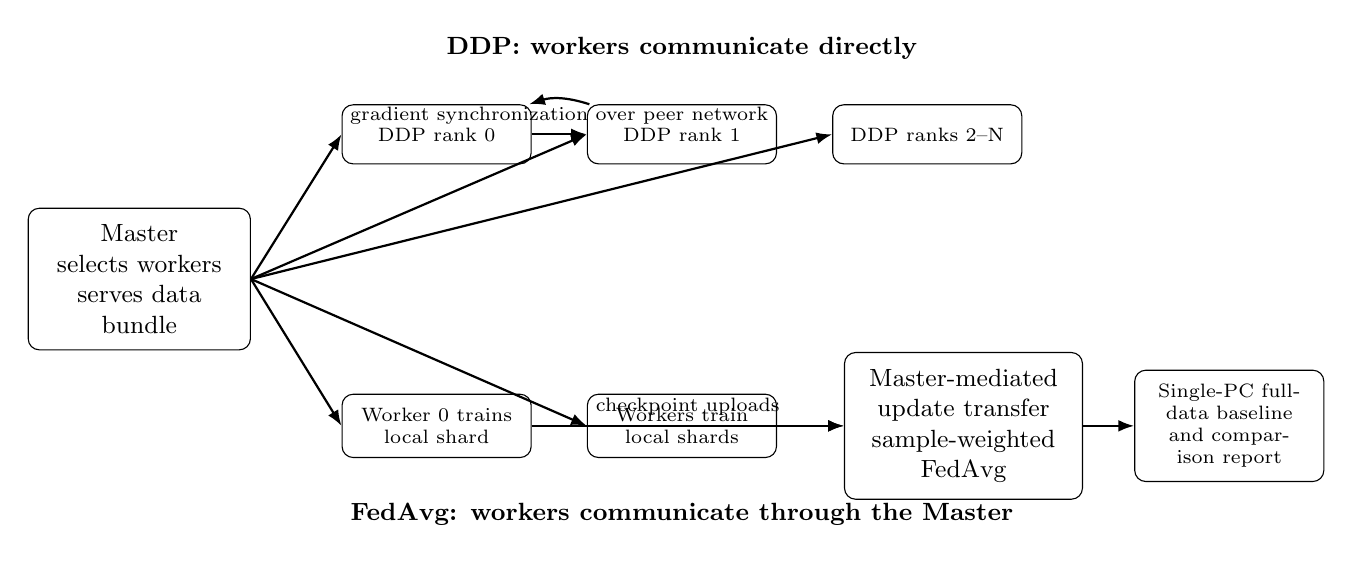
\begin{tikzpicture}[node distance=0.75cm and 0.8cm]
  \node[reportbox,text width=2.4cm] (master) {Master\\selects workers\\serves data bundle};
  \node[reportsmall,above right=0.55cm and 1.15cm of master] (d0) {DDP rank 0};
  \node[reportsmall,right=0.7cm of d0] (d1) {DDP rank 1};
  \node[reportsmall,right=0.7cm of d1] (dn) {DDP ranks 2--N};
  \draw[reportarrow] (master.east) -- (d0.west);
  \draw[reportarrow] (master.east) -- (d1.west);
  \draw[reportarrow] (master.east) -- (dn.west);
  \draw[reportarrow] (d0) -- node[above,font=\scriptsize]{gradient synchronization over peer network} (d1);
  \draw[reportarrow] (d1) to[bend right=18] (d0);
  \node[reportsmall,below right=0.55cm and 1.15cm of master] (f0) {Worker 0 trains local shard};
  \node[reportsmall,right=0.7cm of f0] (f1) {Workers train local shards};
  \node[reportbox,text width=2.6cm,right=0.85cm of f1] (aggregate) {Master-mediated update transfer\\sample-weighted FedAvg};
  \node[reportsmall,right=0.65cm of aggregate] (baseline) {Single-PC full-data baseline\\and comparison report};
  \draw[reportarrow] (master.east) -- (f0.west);
  \draw[reportarrow] (master.east) -- (f1.west);
  \draw[reportarrow] (f0.east) -- node[above,font=\scriptsize]{checkpoint uploads} (aggregate.west);
  \draw[reportarrow] (f1.east) -- (aggregate.west);
  \draw[reportarrow] (aggregate) -- (baseline);
  \node[above=0.45cm of d1,font=\small\bfseries] {DDP: workers communicate directly};
  \node[below=0.45cm of f1,font=\small\bfseries] {FedAvg: workers communicate through the Master};
\end{tikzpicture}
\caption{The two distributed-training workflows supported by IdleGrid.}
\label{fig:training-modes}
\end{figure}

\begin{figure}[htbp]
\centering
\missingfigure{5cm}{Insert a chart generated from repeated lab measurements. Recommended chart: single-PC baseline training time versus FedAvg distributed phase time and end-to-end run time for 2, 3, 5, 10, and selected larger worker counts. Use the same dataset, model, and epoch count. Include actual values and error bars; omit configurations not tested.}
\caption{Performance comparison to be generated from repeated recorded trials.}
\label{fig:results-chart}
\end{figure}

The interpretation of these measurements should separate scheduler overhead from workload execution and report whether any apparent improvement is repeatable. A higher worker count does not necessarily reduce runtime for a small workload because startup, bundle transfer, aggregation, and network overhead may dominate. Any owner-impact conclusion must be based on a controlled observation rather than inferred from the presence of Docker limits.

The analysis should answer the question represented by each experiment rather than merely restating a table. If assignment delay rises with worker count, inspect Master scheduling and heartbeat processing; if container makespan changes, consider CPU contention, memory pressure, input/output behavior, and hardware differences. If a DDP run with more workers is slower, discuss synchronization, image startup, and peer-network overhead. If FedAvg is slower, distinguish local training from bundle/checkpoint transfer, waiting, and aggregation. If replicas are not created, distinguish insufficient worker disk from offline workers, delayed polling, or transfer failure. Discuss both expected behavior and surprises, and include unsuccessful runs as operational evidence.

\textbf{Threats to validity.} A small number of lab machines cannot establish datacenter-scale behavior. Heterogeneous hardware and background user activity can confound comparisons. Image pulls and training-bundle uploads can dominate short-run times. Clock differences across PCs can distort timestamps unless time synchronization is verified; prefer Master-side timestamps for cross-node lifecycle measures where possible. Network congestion, Wi-Fi isolation, firewall rules, and Docker host networking affect DDP independently of compute capacity. Finally, a synthetic image-classification bundle validates the workflow but does not establish model quality on a real application dataset.

	\subsection{Summary of Performance Study}

The available log confirms one three-worker FedAvg workflow completed, but it is not enough to determine whether FedAvg is faster or scales effectively. The 900-image single-PC comparison and repeated worker-count trials remain to be collected. The ordinary scheduler scans registered nodes for each queued job, giving \(O(JN)\) placement work for \(J\) queued jobs and \(N\) nodes in a pass; this is suitable for a small prototype but has not been benchmarked at larger scale.
    
    \subsection{Limitations}
The prototype targets a trusted campus LAN and Windows worker PCs using Docker Desktop and WSL2; results may not generalize to other operating systems, networks, or large clusters. Node, job, booking, student session, and training-run control state is held in memory and is lost when the Master restarts. Student account hashes are file-backed and client endpoints scope jobs and files to the logged-in account, but this is not production-grade authentication. Operator APIs remain sensitive, and worker file replicas are best-effort without repair or rebalance guarantees.

Reported capacity can become stale between heartbeat and scheduling, and first-fit does not provide fairness or optimal packing. Agent activity detection and return-to-active eviction do not guarantee negligible owner impact; an evicted job is failed rather than resumed. Ordinary job output is collected after completion rather than streamed. DDP depends on compatible images, networking, and direct inter-worker TCP connectivity. FedAvg avoids peer TCP but depends on each worker reaching the Master and uses a single aggregation round in this prototype. Performance conclusions remain limited until repeatable measurements are collected on approved lab hardware.

\pagebreak
\section{Conclusions and Future Work}

IdleGrid integrates compute monitoring, first-fit job placement, Docker execution, shared storage, a separate authenticated student client, DDP, and coordinator-mediated FedAvg behind a central Master. One recorded FedAvg run completed across three workers, but no repeated performance trial or 900-image single-PC comparison has yet been recorded. The project therefore demonstrates the workflow, while speedup, scaling, and owner impact still require controlled tests. Constraints include in-memory control state, prototype-level student authentication, approximate resource reports, limited failure recovery, best-effort replicas, and network dependencies.

Future work should run and repeat the 900-image FedAvg comparison at several worker counts, validate the reported metrics, and collect screenshots and logs. Further engineering could strengthen authentication, add durable control records, improve failure recovery and replica repair, and evaluate fairness-aware scheduling such as DRF. DDP reliability could be improved through automated network checks and clearer recovery behavior. Any expansion beyond the campus prototype should evaluate isolation, privacy, resource contention, and administrator approval requirements.

\pagebreak

\section{Scholarly Contributions}
The local Git history records implementation work on shared storage, the DDP and FedAvg workflows, the student client, Master rendezvous/discovery, Agent distribution, and project documentation. The repository is available at \url{https://github.com/avadhutmali/Mega_Project_BTech}. These are collective project outputs; individual member contributions should be added only after the team confirms them.
\begin{enumerate}
\item Research papers: None identified in the repository history; confirm with the team.
\item Patents or copyright: No filing details identified; confirm with the team.
\item Project exhibitions: Add event and date if the team presented the project.
\item Open-source contribution: IdleGrid source repository, \url{https://github.com/avadhutmali/Mega_Project_BTech}. Add the public demo/download URL if required.
\item Certifications: Add relevant verified certificates, if any.
\end{enumerate}


	\pagebreak
	
	\section{References}
	\begin{thebibliography}{9}
\bibitem{condor}
M. Litzkow, M. Livny, and M. Mutka,
\textit{Condor: A Hunter of Idle Workstations},
Proceedings of the 8th International Conference on Distributed Computing Systems, 1988.

\bibitem{boinc}
D. P. Anderson,
\textit{BOINC: A System for Public-Resource Computing and Storage},
Proceedings of the 5th IEEE/ACM International Workshop on Grid Computing, pp. 4--10, 2004.

\bibitem{drf}
A. Ghodsi, M. Zaharia, B. Hindman, A. Konwinski, S. Shenker, and I. Stoica,
\textit{Dominant Resource Fairness: Fair Allocation of Multiple Resource Types},
Proceedings of the 8th USENIX Symposium on Networked Systems Design and Implementation, 2011.

\bibitem{bubbleup}
J. Mars, L. Tang, R. Hundt, S. Skadron, and M. L. Soffa,
\textit{Bubble-Up: Increasing Utilization in Modern Warehouse Scale Computers via Sensible Co-locations},
Proceedings of the 44th Annual IEEE/ACM International Symposium on Microarchitecture, 2011.

\bibitem{heracles}
A. Lo, L. Cheng, R. Govindaraju, P. Ranganathan, and C. Kozyrakis,
\textit{Heracles: Improving Resource Efficiency at Scale},
Proceedings of the 42nd Annual International Symposium on Computer Architecture, 2015.

\bibitem{borg}
B. Burns, B. Grant, D. Oppenheimer, E. Brewer, and J. Wilkes,
\textit{Borg, Omega, and Kubernetes},
Communications of the ACM, vol. 59, no. 5, 2016.

\bibitem{pytorchddp}
PyTorch Contributors,
\textit{DistributedDataParallel},
PyTorch Documentation, available at \url{https://pytorch.org/docs/stable/generated/torch.nn.parallel.DistributedDataParallel.html}.

\bibitem{idlegridguide}
IdleGrid project team,
\textit{IdleGrid -- Project and Technical Guide},
Project repository documentation, DETAILED\_README.md.
\end{thebibliography} 

\pagebreak
\appendix
\section{Appendix A: API and Data-Flow Reference}
This appendix summarizes the implemented Master API surfaces described in the project technical guide. It is included to support system understanding and testing; exact field validation and response structures should be checked against the running version of the repository.

\begin{table}[h!]
\centering
\caption{Node and ordinary-job API summary.}
\label{tab:api-jobs}
\begin{tabular}{|p{0.22\linewidth}|p{0.28\linewidth}|p{0.36\linewidth}|}
\hline
Method and path & Caller & Purpose \\
\hline
\texttt{POST /nodes/heartbeat} & Agent & Create or refresh node capacity and last-seen status \\
\hline
\texttt{GET /nodes/summary} & Dashboard & List known node records and reported status/capacity \\
\hline
\texttt{POST /jobs/submit} & Dashboard/test client & Create a job and immediately attempt scheduling \\
\hline
\texttt{GET /jobs} & Dashboard & List jobs held by the current Master process \\
\hline
\texttt{GET /jobs/\{id\}/status} & Dashboard & Read one job's state, assignment, and result \\
\hline
\texttt{POST /jobs/\{id\}/running} & Agent & Report container start and related runtime information \\
\hline
\texttt{POST /jobs/\{id\}/complete} & Agent & Report result and success/failure outcome \\
\hline
\texttt{GET /agent/\{nodeId\}/assignment} & Agent & Pull an assignment; no assignment is returned as an empty response \\
\hline
\end{tabular}
\end{table}

\begin{table}[h!]
\centering
\caption{Student-client and federated-training API summary.}
\label{tab:api-client-training}
\begin{tabular}{|p{0.34\linewidth}|p{0.2\linewidth}|p{0.34\linewidth}|}
\hline
Method and path & Caller & Purpose \\
\hline
\texttt{POST /client/auth/login} & Student client & Authenticate a configured student account \\
\hline
\texttt{GET /client/nodes} & Student client & Read live lab capacity summary \\
\hline
\texttt{GET /client/jobs} & Student client & List only the signed-in student's jobs \\
\hline
\texttt{POST /client/jobs} & Student client & Submit a resource-limited student job \\
\hline
\texttt{POST /client/jobs/\{id\}/cancel} & Student client & Cancel/release an owned job \\
\hline
\texttt{GET/POST /client/storage/files} & Student client & List owned uploads or upload an owned file \\
\hline
\texttt{GET /client/storage/files/\{key\}/content} & Student client & Download an owned file \\
\hline
\texttt{POST/GET /client/training/runs} & Student client & Submit a student DDP run or list per-user training history \\
\hline
\texttt{POST /federated-training/runs} & Operator dashboard & Submit FedAvg and reserve 2--20 workers \\
\hline
\texttt{GET /federated-training/runs/\{id\}/report} & Operator dashboard & Download per-worker metrics, comparison, and timing \\
\hline
\texttt{GET /federated-training/runs/\{id\}/artifact} & Operator dashboard & Download the aggregated model \\
\hline
\end{tabular}
\end{table}

The student client uses session authentication and backend ownership checks. Student account hashes are file-backed, while sessions, job ownership, and training-history records are in memory for the Master process lifetime. The endpoint list is a summary; request/response schemas should be checked against the running implementation.

\begin{table}[h!]
\centering
\caption{Storage and distributed-training API summary.}
\label{tab:api-storage}
\begin{tabular}{|p{0.22\linewidth}|p{0.28\linewidth}|p{0.36\linewidth}|}
\hline
Method and path & Caller & Purpose \\
\hline
\texttt{GET /storage/summary} & Dashboard & Summarize Master/worker disk capacity and file count \\
\hline
\texttt{GET /storage/files} & Dashboard & List file metadata and access keys \\
\hline
\texttt{POST /storage/files} & Dashboard & Upload multipart file to Master storage \\
\hline
\texttt{GET /storage/files/\{key\}/content} & Browser/user & Download Master-stored content by key \\
\hline
\texttt{GET /agent/\{nodeId\}/storage/assignment} & Agent & Pull a file replica task \\
\hline
\texttt{GET /agent/storage/\{key\}/content} & Agent & Download source bytes for a replica \\
\hline
\texttt{POST /agent/\{nodeId\}/storage/\{key\}/complete} & Agent & Acknowledge replica placement result \\
\hline
\texttt{POST /distributed-training/runs} & Dashboard & Submit a validated bundle and worker configuration \\
\hline
\texttt{GET /distributed-training/runs/\{runId\}} & Dashboard & Read run and per-worker/rank status \\
\hline
\texttt{GET /distributed-training/runs/\{runId\}/bundle} & Worker container & Download the submitted training bundle \\
\hline
\texttt{POST /distributed-training/runs/\{runId\}/artifact} & Rank zero & Upload the final model artifact \\
\hline
\texttt{GET /distributed-training/runs/\{runId\}/artifact} & Dashboard/user & Download the completed artifact \\
\hline
\end{tabular}
\end{table}

The Master HTTP API uses port 9090 by default. Local Agent discovery uses UDP port 9091, and the default DDP rendezvous port is TCP 29500. DDP workers may need additional direct connections. FedAvg worker containers instead contact the Master over HTTP for bundle and update transfers. A successful heartbeat does not establish that peer-to-peer DDP traffic is permitted.

\pagebreak
\section{Appendix B: Deployment and Experiment Record}
The following checklist is intended for an authorized lab setup and a repeatable demonstration. It is not a substitute for institutional approval, security review, or examination of the setup script before running it with administrator privileges.

\textbf{Pre-deployment checklist:}
\begin{enumerate}
  \item Obtain approval to install and run the Agent on each selected PC and to run Docker Desktop/WSL2.
  \item Select one Master and label the worker nodes; record hardware, OS, Java, Docker Desktop, and network information in Table~\ref{tab:environment}.
  \item Start the Master and verify the backend is listening on the configured TCP port. Confirm its advertised LAN URL is reachable from each worker.
  \item Install Java 17+ and Docker Desktop with WSL2 on each worker. Run the provided setup helper only after reviewing its effects and coordinating any required restart.
  \item Configure automatic or manual Master discovery, start each Agent, and verify heartbeat visibility in the dashboard and Master logs.
  \item Pull or locally build the exact ordinary-job, DDP, and FedAvg image versions required by the test. Record the digest and verify image availability before the run.
  \item For DDP, verify peer TCP reachability among selected workers. For FedAvg, verify every selected worker can reach the Master API.
  \item Use non-sensitive synthetic test data and keep operator APIs on the approved campus network. Student login provides prototype account separation but is not a production security boundary.
\end{enumerate}

\textbf{Per-trial record (copy one record for each run):}
\begin{table}[h!]
\centering
\caption{Blank experimental trial record.}
\label{tab:trial-record}
\begin{tabular}{|p{0.35\linewidth}|p{0.5\linewidth}|}
\hline
Field & Value to record \\
\hline
Trial ID / date / operator & [Complete] \\
\hline
Master and worker labels & [Complete] \\
\hline
Software and image versions & [Complete] \\
\hline
Workload / command / input checksum & [Complete] \\
\hline
Requested CPU / memory / worker count & [Complete] \\
\hline
Image cache state / network notes & [Complete] \\
\hline
Job ID or DDP run ID & [Complete] \\
\hline
Submission / assignment / start / finish times & [Complete] \\
\hline
Final status and output/artifact verification & [Complete] \\
\hline
Errors, logs, exclusions, or deviations & [Complete] \\
\hline
\end{tabular}
\end{table}

\textbf{Evidence to include in the final submitted copy:} genuine screenshots of the operator dashboard and student client; a redacted live node summary; a completed job's state and output; a student file upload/download ownership check; a DDP status/artifact if tested; and a FedAvg JSON report showing the distributed run and single-PC baseline. Add the measured comparison chart only after collecting repeat trials. Replace each bracketed field with verified information or mark the test as not performed. Submit institution-required plagiarism and AI-content similarity documents separately from this project report; do not include them as a project chapter. Leave dates and signatures for the team and guide to complete by hand.

\end{document}
